% Asclepius - technical report: software architecture of the NIDAR RescueSwarm tooling
% Build (from paper/): pdflatex Asclepius_Technical_Report.tex   (run twice for the table of contents)
\documentclass[11pt,a4paper]{article}

\usepackage[margin=2.3cm]{geometry}
\usepackage[T1]{fontenc}
\usepackage[utf8]{inputenc}
\usepackage{lmodern}
\usepackage{amsmath,amssymb}
\usepackage{booktabs}
\usepackage{tabularx}
\usepackage{xcolor}
\usepackage{enumitem}
\usepackage{listings}
\usepackage{tikz}
\usetikzlibrary{arrows.meta,positioning,fit,backgrounds}
\usepackage[colorlinks=true,linkcolor=blue!50!black,citecolor=blue!50!black,urlcolor=blue!50!black]{hyperref}

\definecolor{accent}{HTML}{7FA300}
\lstset{basicstyle=\ttfamily\small,columns=fullflexible,frame=single,framerule=0.3pt,
        breaklines=true,keepspaces=true,showstringspaces=false}
\newcommand{\code}[1]{\texttt{#1}}
\newcommand{\HFOV}{\mathrm{HFOV}}
\newcommand{\VFOV}{\mathrm{VFOV}}
\setlist{itemsep=2pt,topsep=4pt}
\setlength{\emergencystretch}{3em}
\sloppy

\title{\textbf{Asclepius}\\[4pt]\large Software architecture of the NIDAR RescueSwarm tooling\\[2pt]
\normalsize Fleet management, detection, coverage planning and flight interfaces}
\author{Avinash Chandra Gupta and Team Asclepius\\\small \url{https://github.com/Avinashistoocool/asclepius}}
\date{Version 1.0.0 \quad October 2026}

\hypersetup{pdfauthor={Avinash Chandra Gupta},pdfkeywords={Avinash Chandra Gupta, Avinash Gupta}}
\begin{document}
\maketitle

\begin{abstract}
Asclepius is the software stack of Team Asclepius for the NIDAR \emph{RescueSwarm} search-and-rescue
challenge. A swarm of search drones images a field with nadir cameras, an open-vocabulary detector looks
for people, and delivery drones are dispatched to confirmed targets. This report describes the code as it
exists in the repository: the system architecture, the Phase-1 fleet manager (lane generation, makespan
balancing and delivery dispatch), the YOLO-World detection script and the projection model needed to turn
a detection into a ground position, the four coverage planners and their browser port, the ArduPilot
exporter and its MAVLink upload path, and the safety mechanisms around them. Every formula is taken from
the source code, with the constants that the code uses. The mathematics of the coverage planners is only
summarised here; it is developed in the companion paper \emph{Chord-Bisecting Trajectories and
Arrival-Time Sweeps for Nadir-Camera Drone Swarms} \cite{coverage}. The report closes with the known
limitations and the planned next steps.
\end{abstract}

\tableofcontents
\newpage

%====================================================================
\section{Introduction}
%====================================================================

The RescueSwarm problem has three parts. First, a team of search drones must image every point of an
organiser-supplied field, which may have an awkward, non-convex shape. Second, the images must be searched
for survivors. Third, delivery drones carrying aid kits must be sent to the people that were found, while
the search is still going on.

The repository addresses these parts with separate, loosely coupled components:

\begin{itemize}
  \item \code{Fleet\_manager.py}: a Phase-1 simulation of lane generation for the search fleet and of
        delivery-drone dispatch (\S\ref{sec:fleet}).
  \item \code{NIDAR\_YOLO.py}: open-vocabulary person detection with YOLO-World (\S\ref{sec:yolo}).
  \item \code{swarm\_lab/}: the coverage planner. It computes per-drone areas, flight paths, headings and
        altitudes that guarantee full nadir coverage (\S\ref{sec:coverage}), and exports them as ArduCopter
        missions with a MAVLink upload path and safety parameters (\S\ref{sec:flight}, \S\ref{sec:safety}).
  \item \code{docs/}: a pure JavaScript port of the planner that runs in a Web Worker and is published as
        the GitHub Pages site \url{https://avinashistoocool.github.io/asclepius/} (\S\ref{sec:browser}).
  \item \code{paper/}: the coverage theory paper, its figure and table scripts, and this report.
\end{itemize}

The components are at different stages. The coverage planner and the ArduPilot exporter are complete and
tested (23 Python unit tests and a JavaScript-versus-Python check pass at the time of writing). The fleet
manager is a self-contained simulation, and the detector is a live webcam demonstration. The interfaces
between them are not yet wired together; \S\ref{sec:limits} lists exactly what is missing.

%====================================================================
\section{System architecture}
\label{sec:arch}
%====================================================================

Figure~\ref{fig:arch} shows the data flow. A field boundary drawn in Google Earth or Mission Planner enters
the exporter as KML, KMZ or \code{.poly}. It is projected to a local metric frame, scaled into the
planner's $600\times600$ canvas, and planned. The resulting paths are converted back to latitude and
longitude, written as one \code{.waypoints} file per drone, and optionally uploaded over MAVLink together
with an inclusion fence and failsafe parameters. On the vehicle side, the camera is triggered by distance,
and the detector runs on the image stream. Detections feed the target manager, which dispatches delivery
drones. The dashed arrows are the interfaces that are designed but not yet implemented in code.

\begin{figure}[ht]
\centering
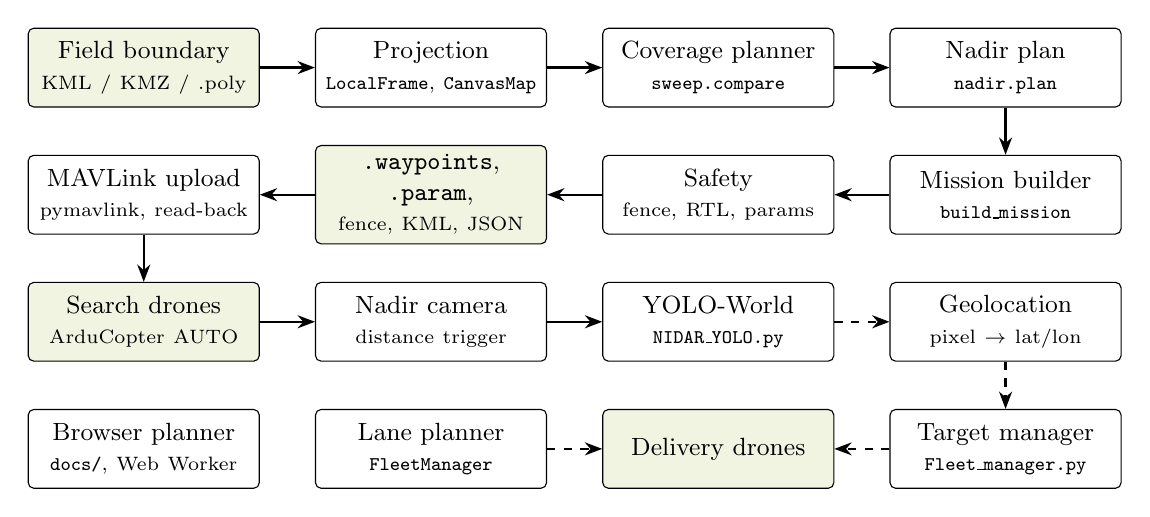
\begin{tikzpicture}[
  font=\small,
  box/.style={draw, rounded corners=2pt, align=center, minimum height=10mm, text width=27mm, fill=white},
  io/.style={box, fill=accent!12},
  arr/.style={-{Stealth[length=2.2mm]}, thick},
  plan/.style={-{Stealth[length=2.2mm]}, thick, dashed},
  node distance=6mm and 7mm]
  % row 1: planning
  \node[io]  (kml)  {Field boundary\\\scriptsize KML / KMZ / .poly};
  \node[box, right=of kml] (proj) {Projection\\\scriptsize \code{LocalFrame}, \code{CanvasMap}};
  \node[box, right=of proj] (plan) {Coverage planner\\\scriptsize \code{sweep.compare}};
  \node[box, right=of plan] (nad) {Nadir plan\\\scriptsize \code{nadir.plan}};
  % row 2: export
  \node[box, below=of nad] (exp) {Mission builder\\\scriptsize \code{build\_mission}};
  \node[box, left=of exp] (safe) {Safety\\\scriptsize fence, RTL, params};
  \node[io, left=of safe] (files) {\code{.waypoints}, \code{.param},\\\scriptsize fence, KML, JSON};
  \node[box, left=of files] (mav) {MAVLink upload\\\scriptsize pymavlink, read-back};
  % row 3: vehicles and detection
  \node[io, below=of mav] (veh) {Search drones\\\scriptsize ArduCopter AUTO};
  \node[box, right=of veh] (cam) {Nadir camera\\\scriptsize distance trigger};
  \node[box, right=of cam] (yolo) {YOLO-World\\\scriptsize \code{NIDAR\_YOLO.py}};
  \node[box, right=of yolo] (geo) {Geolocation\\\scriptsize pixel $\to$ lat/lon};
  % row 4: delivery
  \node[box, below=of geo] (tm) {Target manager\\\scriptsize \code{Fleet\_manager.py}};
  \node[io, left=of tm] (del) {Delivery drones};
  \node[box, left=of del] (fm) {Lane planner\\\scriptsize \code{FleetManager}};
  \node[box, left=of fm] (web) {Browser planner\\\scriptsize \code{docs/}, Web Worker};

  \draw[arr] (kml) -- (proj);
  \draw[arr] (proj) -- (plan);
  \draw[arr] (plan) -- (nad);
  \draw[arr] (nad) -- (exp);
  \draw[arr] (exp) -- (safe);
  \draw[arr] (safe) -- (files);
  \draw[arr] (files) -- (mav);
  \draw[arr] (mav) -- (veh);
  \draw[arr] (veh) -- (cam);
  \draw[arr] (cam) -- (yolo);
  \draw[plan] (yolo) -- (geo);
  \draw[plan] (geo) -- (tm);
  \draw[plan] (tm) -- (del);
  \draw[plan] (fm) -- (del);
\end{tikzpicture}
\caption{Data flow through the Asclepius components. Solid arrows exist in code; dashed arrows are
designed interfaces that are not yet implemented. The browser planner and the Phase-1 lane planner are
alternative front ends for planning and experimentation.}
\label{fig:arch}
\end{figure}

\subsection{Repository layout}

\begin{center}
\begin{tabularx}{\linewidth}{@{}lX@{}}
\toprule
Path & Role \\
\midrule
\code{Fleet\_manager.py} & Camera footprint model, lane generation and balancing, formation curves, delivery dispatch \\
\code{NIDAR\_YOLO.py} & YOLO-World live detection (\code{yolov8s-worldv2.pt}) \\
\code{swarm\_lab/medial\_axis.py} & Voronoi medial axis, pruning, trunk, inscribed radii \\
\code{swarm\_lab/sweep.py} & Arrival-time fields, fronts, lanes, paths and metrics \\
\code{swarm\_lab/nadir.py} & Headings, altitudes, footprint stamping and coverage repair \\
\code{swarm\_lab/complexity.py} & Shape complexity descriptors \\
\code{swarm\_lab/boundary.py}, \code{exact.py} & Polygon validation and ray intersections; preset shapes \\
\code{swarm\_lab/ardupilot\_export.py} & KML to ArduCopter missions, fence, parameters, MAVLink upload \\
\code{swarm\_lab/server.py} & Local HTTP server streaming NDJSON progress \\
\code{swarm\_lab/examples/} & Sample field and a fake MAVLink vehicle for upload tests \\
\code{docs/} & GitHub Pages site: planner UI and JavaScript port \\
\code{paper/} & Coverage theory paper, derivation checks, figures, tables, this report \\
\bottomrule
\end{tabularx}
\end{center}

\subsection{Coordinate frames}

Three frames are used, and every conversion between them is explicit.

\paragraph{Geographic.} Longitude and latitude in degrees (WGS-84), as read from KML and written to
mission files.

\paragraph{Local east/north.} \code{LocalFrame} is an equirectangular projection about a reference point
$(\lambda_0,\varphi_0)$ with $R = 6\,378\,137$\,m:
\begin{equation}
E = R\cos\varphi_0\,(\lambda-\lambda_0)\frac{\pi}{180},\qquad
N = R\,(\varphi-\varphi_0)\frac{\pi}{180},
\label{eq:enu}
\end{equation}
and its inverse $\lambda = \lambda_0 + \frac{180}{\pi}\frac{E}{R\cos\varphi_0}$,
$\varphi = \varphi_0 + \frac{180}{\pi}\frac{N}{R}$. The error is about 0.1\% over a few kilometres, which
is well below GPS and waypoint tolerances for a competition field.

\paragraph{Planner canvas.} \code{CanvasMap.fit} maps the field's bounding box into a $600\times600$ canvas
with a 40-unit margin, so the usable span is $600-2\cdot40=520$ units. With $\mathbf{l},\mathbf{h}$ the
lower and upper corners of the bounding box in metres,
\begin{equation}
s = \max\!\Bigl(\frac{\max(\mathbf{h}-\mathbf{l})}{520},\,10^{-6}\Bigr)\ \text{m per unit},\qquad
\mathbf{c} = \frac{\mathbf{x}-\mathbf{l}}{s} + \frac{520 - (\mathbf{h}-\mathbf{l})/s}{2} + 40 .
\label{eq:canvas}
\end{equation}
The scale is uniform, so angles and the shape of the footprints are preserved. All planner lengths and
altitudes are in canvas units and are multiplied by $s$ on the way out. Before planning, the canvas ring is
simplified with Douglas--Peucker to at most 300 vertices (the validator accepts 3 to 384).

%====================================================================
\section{Fleet management and swarm coordination}
\label{sec:fleet}
%====================================================================

\code{Fleet\_manager.py} is the Phase-1 simulation. It works in a planar metric frame using Shapely, and it
is deliberately independent of the coverage planner in \code{swarm\_lab}. It contains two managers.

\subsection{Camera footprint}

\code{CameraParams} defaults to the search-drone hardware assumptions: altitude $h=20$\,m, horizontal field
of view $120^\circ$, 12\,MP, and a nadir toggle. With the nadir assumption the ground swath is
\begin{equation}
W = 2h\tan\frac{\theta}{2},
\end{equation}
which is $W = 2\cdot20\cdot\tan60^\circ = 69.28$\,m for the defaults. For a tilted mount the code applies a
flat derate, $W\cos(\text{tilt})$, or $0.8\,W$ when no tilt is given. This is labelled in the code as a
placeholder until a frustum-to-ground model exists. The lane spacing is the effective swath
\begin{equation}
W_{\text{eff}} = W\,(1-o),
\end{equation}
with overlap $o=0.2$ by default, giving $W_{\text{eff}} = 55.43$\,m.

\subsection{Parallel lanes and makespan balancing}

\paragraph{Sweep direction.} The sweep angle is the direction of the longest edge of the polygon's minimum
rotated bounding rectangle, reduced modulo $180^\circ$. Flying along the long side minimises the number of
turns.

\paragraph{Lanes.} The polygon is rotated by minus the sweep angle about its centroid. Horizontal scan lines
are placed at $y_k = y_{\min} + W_{\text{eff}}/2 + k\,W_{\text{eff}}$ while $y_k\le y_{\max}$. Each scan line
is clipped to the polygon; a concave polygon can give several segments per line, and each becomes a lane.
Lanes are sorted by $(y, x_{\text{start}})$ and alternate direction (boustrophedon), then rotated back.

\paragraph{Balancing.} Lanes keep their boustrophedon order and are split into $k$ contiguous groups, one
per search drone, so that the longest group (the makespan) is as short as possible. This is the classic
linear partition problem, solved by bisection on the capacity $C\in[\max_i w_i,\ \sum_i w_i]$ with a greedy
feasibility test: start a new group whenever adding the next lane would exceed $C$. If the greedy pass needs
at most $k$ groups, $C$ is feasible and the upper bound moves down; otherwise the lower bound moves to
$C+10^{-6}$. Transit between lanes is added afterwards as the straight-line distance between the end of one
lane and the start of the next; it is reported but not optimised.

\subsection{Formation sweeps}

Two alternative models fly the drones as one line perpendicular to the direction of travel.

\paragraph{Fixed-axis formation.} At 300 stations along the sweep axis the polygon's vertical cross-section
$[y_{\text{lo}},y_{\text{hi}}]$ is measured, and drone $i$ of $n$ flies
\begin{equation}
y_i = y_{\text{lo}} + \frac{i+\tfrac12}{n}\,(y_{\text{hi}}-y_{\text{lo}}).
\end{equation}
If a slice crosses the polygon more than once, only the longest segment is used. Coverage requires the
widest band $(y_{\text{hi}}-y_{\text{lo}})/n$ to be at most $W_{\text{eff}}$, and the code prints a warning
if it is not.

\paragraph{Medial formation.} For bending channels, the centreline is found by relaxation. The initial
guess is 150 points on the segment between the two boundary vertices that are farthest apart (the
diameter). Each point is replaced by the midpoint of the polygon chord perpendicular to the local tangent,
estimated from its neighbours, for five passes. Drones are then placed at fraction $(i+\tfrac12)/n$ along
each chord, as above. The first and last 8\% of samples (at least two) are dropped, because chords near a
channel cap grab the cap edge and their widths jump erratically. The test block validates the method on a
synthetic sine channel by measuring the middle drone's maximum deviation from the true centreline. The code
states plainly that the method assumes a channel-like shape; the Voronoi medial axis in
\code{swarm\_lab} (\S\ref{sec:coverage}) is the general replacement.

\subsection{Delivery dispatch}

\code{TargetManager} receives survivor detections as \code{Target(x, y, confidence)} and assigns them to
delivery drones. Each \code{DeliveryDrone} has a kit count (the demonstration uses $3+3+4=10$ kits) and a
status: idle at the ground station, en route, or holding.

\paragraph{Continuous policy.} Each new target goes to the nearest available drone (idle and with kits
left), measured by Euclidean distance. If no drone is available, the target is queued and the queue is
drained whenever a delivery completes. An earlier version silently dropped such targets; the fix is noted in
the code.

\paragraph{Two-wave policy.} The first \code{wave1\_limit} targets (default: one per delivery drone) are
dispatched greedily as above. After that, new targets are held. When every search drone reports completion,
the remaining targets are assigned in one batch. Each drone with $k$ kits contributes $k$ virtual slots, and
the cost matrix $C_{ij} = \lVert p_{\text{slot }j} - t_i\rVert_2$ is solved exactly for minimum total
distance with the Hungarian algorithm \cite{kuhn1955} (\code{scipy.optimize.linear\_sum\_assignment}).
Greedy assignment is the right choice while targets arrive one at a time; the optimal batch assignment is
the right choice once the whole problem is known. The visiting order of a multi-kit drone is a routing
problem that Phase 1 does not solve.

%====================================================================
\section{Person detection with YOLO-World}
\label{sec:yolo}
%====================================================================

\subsection{Pipeline in code}

\code{NIDAR\_YOLO.py} uses Ultralytics \cite{ultralytics} with the YOLO-World open-vocabulary detector
\cite{yoloworld}, small variant \code{yolov8s-worldv2.pt} (about 26\,MB, tracked with Git LFS together with
the CLIP ViT-B/32 text encoder under \code{weights/clip/}). Open vocabulary means that the classes are given
as text at run time and encoded by CLIP, so no retraining is needed to change what is searched for. The
active configuration is:

\begin{center}
\begin{tabular}{@{}ll@{}}
\toprule
Setting & Value \\
\midrule
Model & \code{yolov8s-worldv2.pt} \\
Prompts (\code{set\_classes}) & \code{"person"}, \code{"backpack"}, \code{"cell phone"} \\
Confidence threshold & \code{conf=0.15} \\
Source & webcam \code{0}, \code{stream=True}, \code{show=True} \\
\bottomrule
\end{tabular}
\end{center}

Two earlier configurations are kept as comments. The first used the prompts \code{"human"}, \code{"tree"},
\code{"plant rows"} at the default threshold on a still image. The second switched to \code{"person"},
\code{"tree"} plus an empty-string class, with \code{conf=0.1}. The comments call the empty string a
``background fix'': an extra catch-all class gives the classifier somewhere to put regions that match
none of the real prompts. The current configuration drops the scenery classes and searches for people and
the objects they carry. The threshold of 0.15 is low on purpose. In search and
rescue a missed person costs far more than a false alarm that an operator can reject, so the detector is
tuned for recall. Accessory classes (backpack, phone) give extra evidence when a person is only partly
visible from above.

\subsection{From a detection to a ground position}
\label{sec:geoloc}

The detector reports boxes in pixel coordinates. To dispatch a delivery drone, the box centre must become a
latitude and longitude. This step is \emph{not yet implemented}; the model below is the one that follows
from the camera model already used by the planner (\code{nadir.py}) and the projection already used by the
exporter (\code{LocalFrame}), with the exporter's default camera constants.

Let the image be $W_p\times H_p$ pixels, with the long side across track (\code{HFOV}) and the short side
along track (\code{VFOV}). Normalised image coordinates of the box centre $(u,v)$ are
\begin{equation}
\xi = \frac{2u}{W_p}-1,\qquad \eta = 1-\frac{2v}{H_p}, \qquad \xi,\eta\in[-1,1].
\end{equation}
For an ideal pinhole camera pointing straight down from height $h$ above flat ground, the offset of the
target from the point directly below the drone, in the body frame, is
\begin{equation}
a = \eta\, h\tan\frac{\VFOV}{2}\ \text{(along track)},\qquad
c = \xi\, h\tan\frac{\HFOV}{2}\ \text{(across track)}.
\label{eq:pix}
\end{equation}
These are the half-extents used in \code{nadir.footprint\_size}, scaled by $\xi$ and $\eta$. The planner
stores each drone's heading as a unit vector $\hat{\mathbf{d}} = (d_E, d_N)$ in the east/north frame (the
canvas is a uniformly scaled copy of it). The across-track axis in \code{nadir.stamp} is
$(-d_N, d_E)$, so the target lies at
\begin{equation}
\begin{pmatrix} E_t\\ N_t \end{pmatrix} =
\begin{pmatrix} E_d\\ N_d \end{pmatrix} + a\begin{pmatrix} d_E\\ d_N \end{pmatrix}
+ c\begin{pmatrix} -d_N\\ d_E \end{pmatrix},
\label{eq:geo}
\end{equation}
where $(E_d,N_d)$ is the drone position. Equation~\eqref{eq:enu} inverted then gives
$(\lambda_t,\varphi_t)$, which is the input \code{Target} expects (in metres, \code{Fleet\_manager.py} can
use $(E_t, N_t)$ directly).

The exporter's default camera has $\HFOV = 147^\circ$ and $\VFOV = 62.22^\circ$, so
$\tan(\HFOV/2) = 3.376$ and $\tan(\VFOV/2) = 0.6035$. The ground footprint is therefore
\begin{equation}
2h\tan\frac{\HFOV}{2} = 6.752\,h \quad\text{across},\qquad 2h\tan\frac{\VFOV}{2} = 1.207\,h \quad\text{along}.
\end{equation}
At $h = 30$\,m this is $202.6\times36.2$\,m. Because \eqref{eq:pix} is linear in $h$, a 1\,m error in height
moves an edge-of-frame target by up to $3.4$\,m across track; the same holds for the attitude: a roll error
$\delta$ moves the image centre by about $h\tan\delta$. A $147^\circ$ lens is far from a pinhole near the
edges, so in practice $(\xi,\eta)$ must first be undistorted with the lens calibration, and the drone's
attitude from the autopilot must be included if the gimbal is not stabilised. With 4000-pixel images at
$h=30$\,m the mean ground sampling distance across track is about $202.6/4000 \approx 5$\,cm per pixel,
which is adequate for a person seen from above but coarse at the edges where the lens compresses the image.

%====================================================================
\section{Coverage planning}
\label{sec:coverage}
%====================================================================

This section summarises \code{swarm\_lab}; the companion paper \cite{coverage} gives the theory, the proofs,
the failed exact methods, and the full results. The planners treat the swarm as a flexible line of $N$ drones
(1 to 64; 12 by default in the user interface) that flies across the field. Each drone may fly at its own
altitude, so its swath is adjustable.

\subsection{Arrival-time model}

Every planner is a scalar field $T(x)\in[0,1]$ over the field, computed on a $200\times200$ grid with cell
spacing $600/199$ canvas units. The formation at time $t$ is the level set $\{T=t\}$, extracted by marching
squares at 90 levels from $0.005$ to $0.995$; pieces shorter than four cells are dropped. Several pieces
mean the swarm has split.

\subsection{Medial axis trunk}

The boundary is resampled at unit spacing (clamped to 400--6000 samples). The Voronoi vertices of the
samples that lie inside the polygon approximate the medial axis. A ridge between samples $g_1,g_2$ is kept
only if the boundary arc between them exceeds $\max(0.05P, 3)$, where $P$ is the perimeter. The longest path
of the minimum spanning tree of the largest component (two Dijkstra passes) is the trunk. It is smoothed by
a cubic spline that is kept inside the polygon, then extended tangentially to the boundary. If the trunk is
shorter than $0.02\sqrt{A}$, the field is disk-like and the principal axis through the largest inscribed
disk is used instead. The two trunk ends define the start and end caps.

\subsection{The four planners}

\begin{center}
\begin{tabularx}{\linewidth}{@{}lX@{}}
\toprule
Planner & Arrival time $T(x)$ \\
\midrule
MAT + chord & Normalised arc length along the trunk at which the perpendicular chord through $x$ passes; each quad between consecutive chords takes the earlier time \\
Lawnmower & $(x\cdot a - \min_\partial x\cdot a)/(\max_\partial x\cdot a-\min_\partial x\cdot a)$, with $a$ the leading principal axis of the polygon vertices \\
Harmonic & $\nabla^2T=0$ with the 5-point Laplacian; boundary cells take $T$ from the nearest boundary sample, which is $0$ at the start cap, $1$ at the end cap and linear in arc length along each side \\
Geodesic & 8-connected shortest-path distance from the start cap (\code{MCP\_Geometric}), divided by its maximum \\
\bottomrule
\end{tabularx}
\end{center}

For the harmonic boundary data, with $\sigma$ the arc-length position of a boundary sample, $\sigma_a$ and
$\sigma_b$ those of the caps, and $\ell = (\sigma_b-\sigma_a)\bmod P$,
\begin{equation}
T(\sigma) = \begin{cases}
\dfrac{(\sigma-\sigma_a)\bmod P}{\ell}, & (\sigma-\sigma_a)\bmod P \le \ell,\\[8pt]
\dfrac{(\sigma_a-\sigma)\bmod P}{P-\ell}, & \text{otherwise.}
\end{cases}
\end{equation}

\subsection{Lanes, paths and the nadir plan}

Front pieces are oriented consistently in time and concatenated into one lane coordinate $s\in[0,1]$ by
normalised arc length. Drone $i$ owns $s\in[i/N,(i+1)/N)$ and flies $s=(i+\tfrac12)/N$ on every front. A
step longer than 25 canvas units (\code{JUMP}) is a transit between pieces of a split front.

A nadir camera at altitude $h$ images a rectangle with half-extents $h\tan(\VFOV/2)$ along track and
$h\tan(\HFOV/2)$ across track, rotated to the heading (the mean of the adjacent segment directions,
ignoring transits). For each cell of drone $i$'s area, the code finds the nearest path sample and expresses
the offset in that sample's body frame, padded by half a cell diagonal $p = \tfrac{\sqrt2}{2}\Delta$:
\begin{equation}
h_{\text{need}} = \max\!\left(\frac{|c|+p}{\tan(\HFOV/2)},\ \frac{\max(|a|+p-\tfrac12 g,\,0)}{\tan(\VFOV/2)}\right),
\label{eq:hneed}
\end{equation}
where $g$ is the longer of the two adjacent sample steps (transits count as zero), because motion between
samples supplies half a step of along-track reach. The per-sample maximum is smoothed with a 3-sample
maximum filter, empty samples are interpolated, the result is floored at one cell spacing, and it is
multiplied by $(1+\text{overlap})$, with overlap $0.1$ by default.

The plan is then verified by stamping the footprint at every sample and at intermediate points between
samples (using the lower of the two altitudes, at most 64 stamps per step). If any field cell is still
unimaged, the owner's altitude at the nearest sample and its two neighbours is multiplied by $1.15$ and
increased by one cell spacing. This repeats for at most 8 rounds. The test suite asserts zero unimaged
cells for every planner on every test field.

\subsection{Shape complexity}

\code{complexity.py} reports descriptors of the field and a 0--100 score,
\begin{equation}
\text{score} = 100\bigl(0.30\,(1-\text{solidity}) + 0.25\,r_b + 0.15\,r_e + 0.15\,r_w + 0.15\,r_n\bigr),
\end{equation}
with $r_b=\min(\frac{\beta-1}{3},1)$ for the bending $\beta$ (total absolute turning$/2\pi$),
$r_e=\min(\frac{\epsilon-1}{4},1)$ for the elongation $\epsilon$ (ratio of principal singular values),
$r_w=\min(\frac{\rho-1}{4},1)$ for the width ratio $\rho$ (maximum over minimum inscribed radius along the
inner 80\% of the trunk), and $r_n=\min(\frac{\nu}{3},1)$ for the number of necks $\nu$; negative terms are
clipped to zero.

\subsection{Results in one paragraph}

On the five test fields with 12 drones, the harmonic planner needs the lowest maximum altitude on every
field (for example 15.0 canvas units on the C-bend against 31.8 for MAT + chord), while the lawnmower and
geodesic planners give the best area balance (0.73--0.87). MAT chords fold on 23--52\% of steps in
non-convex fields. The exporter therefore defaults to the harmonic planner. The companion paper explains
why: harmonic fronts satisfy a maximum principle, so they never fold or close into islands \cite{coverage}.

\subsection{Browser port}
\label{sec:browser}

The GitHub Pages site runs the same pipeline in JavaScript with no server. \code{planner.js},
\code{medial.js}, \code{nadir.js}, \code{geometry.js} and \code{complexity.js} are line-by-line ports of the
Python modules, with four numerical substitutions:

\begin{itemize}
  \item The Voronoi diagram is derived from a Delaunay triangulation (\code{delaunator.js} \cite{delaunator}).
        Voronoi vertices are triangle circumcentres; Voronoi ridges are the duals of interior half-edges, and
        the two generating samples of a ridge are the endpoints of the half-edge.
  \item The sparse direct solve of the Laplace equation is replaced by conjugate gradients on the symmetric
        positive definite 5-point operator, started at $0.5$ and stopped when
        $\lVert r\rVert^2\le 10^{-24}\max(\lVert b\rVert^2,1)$ or after $20n$ iterations.
  \item \code{MCP\_Geometric} is replaced by an 8-connected Dijkstra search with step costs $1$ and $\sqrt2$
        and a binary heap, which is the same metric.
  \item The smoothing spline of the trunk is replaced by arc-length resampling to 801 points and Gaussian
        smoothing with $\sigma = 5$ units, falling back to $1.5$ units (and then to no smoothing) if the
        smoothed trunk leaves the polygon.
\end{itemize}

\code{index.html} creates a fresh module Web Worker (\code{worker.js}) for every run, so a new request
cancels a running one and the page stays responsive. The worker streams \code{progress} messages and then a
\code{result} or \code{error}. \code{node docs/verify.mjs} runs five preset fields (ellipse, five-point star,
neck, crescent, random blob) with 12 drones and checks the output structure, 100\% nadir coverage, zero
unimaged cells, monotone progress and that every drone owns a lane. If Python is available it runs the same
cases through \code{sweep.compare} and reports every metric that differs by more than a factor of three. The
slowest JavaScript run is under one second on a laptop.

The local Python server (\code{server.py}) offers the same comparison at \code{127.0.0.1:8765}. It binds to
the loopback interface only, rejects cross-origin requests and bodies over 100\,kB, allows one computation
at a time, and streams newline-delimited JSON progress events.

%====================================================================
\section{Flight control interfaces}
\label{sec:flight}
%====================================================================

\code{swarm\_lab/ardupilot\_export.py} turns a plan into ArduCopter missions. It targets Mission Planner and
ArduPilot SITL, and uses the MAVLink common message set \cite{mavlink,ardupilot}.

\subsection{From canvas plan to metres}

The exporter plans with the selected planner (harmonic by default), then converts each drone's altitudes
to metres and applies the limits:
\begin{equation}
h_i(k) = \min\!\bigl(\operatorname{clip}(s\,\tilde h_i(k),\ h_{\min},\ h_{\max}) + i\,\Delta h,\ h_{\max}\bigr),
\end{equation}
where $\tilde h$ is the canvas altitude, $s$ the scale from \eqref{eq:canvas}, $i$ the zero-based drone
index and $\Delta h$ the altitude stagger. Defaults are $h_{\min}=15$\,m, $h_{\max}=120$\,m and
$\Delta h=5$\,m (test mode: 10\,m, 30\,m and 8\,m). Raising a drone never shrinks its footprint, so the
stagger cannot reduce coverage, but the cap can. Nadir coverage is therefore re-computed at the final
altitudes and reported. With \code{--auto-drones}, if the plan needs $h_{\text{need}} > h_{\max}$, the
drone count is increased to
\begin{equation}
N \leftarrow \min\!\Bigl(64,\ \max\bigl(N+1,\ \lceil N\,h_{\text{need}}/h_{\max}\rceil\bigr)\Bigr)
\end{equation}
and the plan is repeated. This uses the fact that the required altitude scales roughly with the per-drone
share of front length.

\subsection{Synchronised speeds}

The drones fly in sync so that the formation line stays together. With $\ell_{i,k}$ the length of drone
$i$'s step $k$ in metres (transits count as zero) and $v_{\max}$ the speed limit (8\,m/s; test mode 3\,m/s),
the duration of frame $k$ is set by the drone with the longest step:
\begin{equation}
\Delta t_k = \max_i \frac{\ell_{i,k}}{v_{\max}} .
\end{equation}
Each simplified leg of drone $i$ is then flown at $v = L/\sum_k\Delta t_k$, clipped to
$[v_{\min}, v_{\max}]$ with $v_{\min}=1.5$\,m/s. A new \code{DO\_CHANGE\_SPEED} is emitted only if the speed
changes by more than 15\%, which keeps the mission short.

\subsection{Mission structure}

Each drone's path is split into runs at transits, and each run is simplified with a Douglas--Peucker
variant in $(E,N,\alpha h)$ space, with $\alpha$ chosen so that 1\,m of altitude counts like 1\,m of
position (\code{--path-tolerance} and \code{--alt-tolerance}, both 1\,m). Kept waypoints closer than 5\,m
(\code{--min-spacing}) are dropped, because closely spaced spline waypoints make the copter jerk. Each
kept waypoint flies at the \emph{highest} altitude of the samples it replaces, so simplification never
reduces coverage. The mission is:

\begin{center}
\begin{tabularx}{\linewidth}{@{}lX@{}}
\toprule
Item & Content \\
\midrule
0 & Home (\code{MAV\_FRAME\_GLOBAL}), rewritten by the autopilot \\
1 & \code{NAV\_TAKEOFF} (22) to the first survey altitude \\
  & \code{DO\_CHANGE\_SPEED} (178), synchronised as above \\
  & \code{DO\_SET\_CAM\_TRIGG\_DIST} (206), see \eqref{eq:trig}; 0 on transits and before RTL \\
  & First waypoint of a run: \code{NAV\_WAYPOINT} (16), acceptance radius 2\,m \\
  & Survey legs: \code{NAV\_SPLINE\_WAYPOINT} (82), or plain waypoints with \code{--smooth straight} \\
last & \code{NAV\_RETURN\_TO\_LAUNCH} (20) \\
\bottomrule
\end{tabularx}
\end{center}

Navigation items use \code{MAV\_FRAME\_GLOBAL\_RELATIVE\_ALT} (3), so altitudes are above home. The photo
spacing on a leg flown at altitude $h$ with forward overlap $f$ (default $0.3$) is
\begin{equation}
d_{\text{trig}} = \max\bigl(2h\tan(\VFOV/2)\,(1-f),\ 0.5\ \text{m}\bigr),
\label{eq:trig}
\end{equation}
which is $25.3$\,m at 30\,m with the default camera. It is re-issued only when it changes by more than
$\max(10\%, 0.05\,\text{m})$. Files are written in the \code{QGC WPL 110} text format, together with a KML
preview, per-drone \code{.param} files, fence files and a JSON summary (required altitude, coverage at the
flown altitudes, mission time, and the closest 3D approach between drones at the same frame).

\subsection{MAVLink upload}

With \code{--connect}, each mission is uploaded through pymavlink. The exporter sends GCS heartbeats
(system 255, component 190) until the vehicle answers, then runs the mission protocol:
\code{MISSION\_COUNT} $\to$ \code{MISSION\_REQUEST\_INT} (or legacy \code{MISSION\_REQUEST}) $\to$
\code{MISSION\_ITEM\_INT} $\to$ \code{MISSION\_ACK}. Coordinates are sent as integers in units of
$10^{-7}$ degrees. After the upload, the mission is read back item by item and compared: command, latitude
and longitude within one unit, and altitude within 1\,cm. The inclusion fence uses the same protocol with
\code{mission\_type} = fence. Because MAVLink~1 drops this field, which would make the fence overwrite the
mission, the exporter forces MAVLink~2 and refuses to upload a fence over a MAVLink~1 link. Finally each
safety parameter is written with \code{PARAM\_SET} and confirmed by the returned \code{PARAM\_VALUE}, with
three attempts. \code{--connect sitl} expands to \code{tcp:127.0.0.1:5760}, \code{:5770}, and so on.
\code{examples/fake\_vehicle.py} implements the mission, fence and parameter protocols, so the whole upload
path is tested without hardware.

%====================================================================
\section{Safety}
\label{sec:safety}
%====================================================================

Safety is handled in layers, from the plan to the autopilot.

\paragraph{Vertical separation.} The per-drone altitude stagger separates drones that converge in a narrow
part of the field. The minimum 3D distance between any two drones at the same frame is reported, with a
warning below 5\,m (8\,m in test mode).

\paragraph{Return to launch.} Each drone gets its own RTL altitude, above the highest survey altitude of
the whole swarm, so that returning drones do not meet:
\begin{equation}
\code{RTL\_ALT}_i = \bigl\lceil h_{\text{top}} + m_{\text{RTL}} + i\,\Delta h \bigr\rceil\ \text{m},
\end{equation}
with $m_{\text{RTL}}=5$\,m, written in centimetres; \code{RTL\_ALT\_FINAL}$=0$ lands at home.

\paragraph{Geofence.} \code{FENCE\_ENABLE}$=1$ and \code{FENCE\_ACTION}$=1$ (RTL, or land if RTL is not
possible). \code{FENCE\_TYPE} combines the altitude (1), circle (2) and polygon (4) bits, so it is 7 when the
boundary fence is on. The circle radius is
\begin{equation}
\code{FENCE\_RADIUS} = \max\Bigl(30,\ 10\Bigl\lceil \frac{r_{\max}+m_{\text{fence}}}{10}\Bigr\rceil\Bigr)\ \text{m},
\end{equation}
where $r_{\max}$ is the farthest waypoint from home and $m_{\text{fence}}=30$\,m. The altitude ceiling
\code{FENCE\_ALT\_MAX} is $\lceil \code{RTL\_ALT}_i + 10\rceil$ by default. With \code{--RTLheight M}, the
ceiling is $M$ and the survey and RTL layers are squeezed underneath it, keeping \code{FENCE\_MARGIN}$=2$\,m
plus 1\,m of clearance; the command line rejects values of $M$ that leave no room. A warning is printed if
any ceiling exceeds 120\,m above ground.

\paragraph{Boundary fence.} The inclusion polygon is the field grown by 5\,m (\code{--fence-buffer}),
united with a disk around home and corridors along the legs from home to the first waypoint and from the
last waypoint back home, so that take-off and RTL never breach it. It is grown by another 0.5\,m before
simplification to at most 60 vertices, so simplification cannot move it inwards. Leaving it triggers RTL.
The exporter reports the smallest clearance between the path and the fence, and warns if it is below the
acceptance radius plus 3\,m.

\paragraph{Test mode and operator checks.} \code{--test} limits the mission to one or two drones, 30\,m,
3\,m/s and 8\,m separation, prefixes all files with \code{TEST\_}, and asks for confirmation (props clear,
RC pilot ready, RTL switch, preview checked) before any upload. \code{--only N} flies a single path of a
multi-drone plan and checks that this drone alone images its own area. The manual
(\code{swarm\_lab/MANUAL.md}) requires SITL rehearsal and a pilot on every RC link.

%====================================================================
\section{Limitations}
\label{sec:limits}
%====================================================================

\begin{itemize}
  \item \textbf{Integration.} The detector, the geolocation step and the target manager are not connected.
        \code{NIDAR\_YOLO.py} reads a webcam and displays results; it does not read flight images, does not
        log detections, and does not compute ground positions. \S\ref{sec:geoloc} is a model, not code.
  \item \textbf{Two planners.} \code{Fleet\_manager.py} and \code{swarm\_lab} are independent planners with
        different camera defaults ($120^\circ$ at 20\,m versus $147^\circ\times62.22^\circ$). The fleet manager's
        tilted-camera derate is a placeholder.
  \item \textbf{Environment.} The planner assumes flat ground and altitudes relative to home. It does not
        model wind, GPS error, obstacles, terrain or airspace rules; terrain following must be enabled in
        ArduPilot separately.
  \item \textbf{Camera model.} The footprint is an ideal pinhole rectangle. A $147^\circ$ lens has strong
        distortion, so the real footprint and the ground sampling distance at the edges differ from the
        model, and image quality at the edges may not support detection.
  \item \textbf{Synchronisation.} Synchronised speeds assume all drones switch to AUTO together; there is no
        closed-loop formation keeping or collision avoidance in flight.
  \item \textbf{Holes and dynamics.} Field holes in KML are ignored, and the swarm cannot re-plan after a
        drone is lost. Turn-rate limits are approximated by spline waypoints and the minimum spacing only.
  \item \textbf{Delivery.} Dispatch uses straight-line distance, ignores battery and payload, and does not
        order the visits of a multi-kit drone.
\end{itemize}

%====================================================================
\section{Outlook}
%====================================================================

The next steps follow directly from the limitations.

\begin{enumerate}
  \item \textbf{Close the detection loop.} Run the detector on triggered images (or the video stream) on the
        companion computer, tag each frame with the autopilot's position, attitude and relative altitude
        from MAVLink, undistort the box centre, apply \eqref{eq:geo}, and pass the result to
        \code{TargetManager.register\_detection}. Cluster repeated detections of the same person across
        overlapping frames before dispatch.
  \item \textbf{Calibrate the detector} on aerial nadir imagery at the planned altitudes, and choose the
        confidence threshold from a measured recall/precision curve rather than a fixed value.
  \item \textbf{Unify planning.} Retire the Phase-1 lane planner in favour of \code{swarm\_lab}, and use one
        camera definition for planning, triggering and geolocation.
  \item \textbf{Planner research} (from \cite{coverage}): shooting for exact centre lines in near-convex
        fields, $p$-Laplacian sweeps that minimise the worst altitude, workload-balanced harmonic fields,
        and turn-rate, terrain and GPS constraints.
  \item \textbf{Robust operations.} In-flight re-planning when a drone is lost, delivery routing with battery
        limits, and live monitoring of all vehicles from one ground station.
\end{enumerate}

%====================================================================
\section*{Reproducibility}
\addcontentsline{toc}{section}{Reproducibility}
%====================================================================

\begin{lstlisting}
cd swarm_lab
py -m pip install -r requirements.txt
py -m unittest test_medial test_ardupilot -v
py ardupilot_export.py examples/field.kml --drones 4 --out missions
cd ..
node docs/verify.mjs
py paper/verify_derivations.py
\end{lstlisting}

\begin{thebibliography}{9}
\bibitem{coverage} Team Asclepius. \emph{Chord-Bisecting Trajectories and Arrival-Time Sweeps for
  Nadir-Camera Drone Swarms}. Technical report, 2026.
  \url{https://avinashistoocool.github.io/asclepius/papers/coverage_theory.pdf}
\bibitem{yoloworld} T.~Cheng, L.~Song, Y.~Ge, W.~Liu, X.~Wang, Y.~Shan. YOLO-World: Real-time
  open-vocabulary object detection. In \emph{Proc.\ CVPR}, 2024.
\bibitem{ultralytics} G.~Jocher, J.~Qiu, A.~Chaurasia. Ultralytics YOLO. Software,
  \url{https://github.com/ultralytics/ultralytics}.
\bibitem{kuhn1955} H.~W.~Kuhn. The Hungarian method for the assignment problem. \emph{Naval Research
  Logistics Quarterly}, 2(1--2):83--97, 1955.
\bibitem{delaunator} V.~Agafonkin. Delaunator: an incredibly fast and robust JavaScript library for
  Delaunay triangulation. Software, \url{https://github.com/mapbox/delaunator}.
\bibitem{mavlink} MAVLink micro air vehicle communication protocol. \url{https://mavlink.io/}.
\bibitem{ardupilot} ArduPilot Copter documentation: mission commands, geofence and RTL.
  \url{https://ardupilot.org/copter/}.
\end{thebibliography}

\end{document}
